\documentclass{article}

\usepackage{graphicx}
\usepackage[T1]{fontenc}
\usepackage[utf8]{inputenc}
\usepackage[francais]{babel}

\title{Simple Count Documentation}
\author{Etienne DEBAS}
\date{23 Novembre 2014}

\begin{document}

\maketitle
\tableofcontents
\newpage
\section{Choix des composants}

	Le package Swing de java a été utilisé pour l'interface homme machine.
	
	\subsection{Ecran}	
	L'ecran de la calculatrice est composé de 3 JTextField permettant :
	\begin{itemize}
	\item[•] d'afficher la totalité l'expression courante.
	\item[•] d'ajouter un élément à l'expression en cours.
	\item[•] d'afficher un message en cas d'erreur.
	\end{itemize}
	
	\subsection{Les buttons}	
	Les bouttons de la calculatrice ont été créés grace à l'objet JButton.\\
	Pour l'insertion des JTextField et des JButton au sein de l'interface j'ai utilisé
	l'objet JPanel avec les conteneur suivant :	
	\begin{itemize}
	\item[•] gridLayout
	\item[•] box
	\item[•] gridBagLayout
	\end{itemize}

	~~\newline
	L'ensemble des composants est mis en place dans une JFrame
\section{Choix du design}
	Trouvant le thème de base proposé par Swing trop clair et trop sobre j'ai choisi de customiser
	la plupart des composants de la calculatrice comprenant les JTextField et les JButton.
	Tous les  éléments ont été initialisés avec un background DARK\_GREY, avec un foreground WHITE
	pour la police et avec une custom font.
	
	Les bordures des JTextField ont été suprimés afin de n'avoir aucune séparation apparente entre eux.
	Les boutons \textbf{Undo} et \textbf{Clear} implémentent des icons permettant de mieux se représenter leurs fonctionnalités.
\section{Conception}

	\subsection{IDE}
	L'IDE Intellij IDEA a été utilisé pour le développement de ce projet	car celui ci propose
	des fonctionnalités très interessante pour l'élabortation d'un projet java :
	\begin{itemize}
	\item[•] une autocomplétion de qualité
	\item[•] une intégration du versionning avec Git
	\item[•] permet de développer du J2EE et de l'android
	\end{itemize}		

	\subsection{Package}
	Les classes ont été placées dans des packages differents afin de gagner en visibilité.\\
	Le package \textbf{ui} regroupe les classes en rapport avec l'interface graphique.\\
	Le package \textbf{math} regroupe l'évaluateur d'expression et les
	unicodes mathématiques pour l'interface graphique.\\
	Le package \textbf{exception} contient la classe d'exception pour l'évaluateur d'expression.\\
	Les packages \textbf{model} et \textbf{controller} regroupent les classes du pattern \textit{\textbf{MVC}}.

	\subsection{Heritage}
	Afin d'éviter les répetitions de code les objets de l'IHM héritent de ceux de Swing afin
	d'initialiser leurs attributs dés leur construction (SimpleCountButton, SimpleCountField)
	Utilisé aussi pour le listener des bouttons, pour l'exception mais aussi pour le pattern \textit{\textbf{MVC}}.

	\subsection{Pattern MVC}	
	\begin{center}
	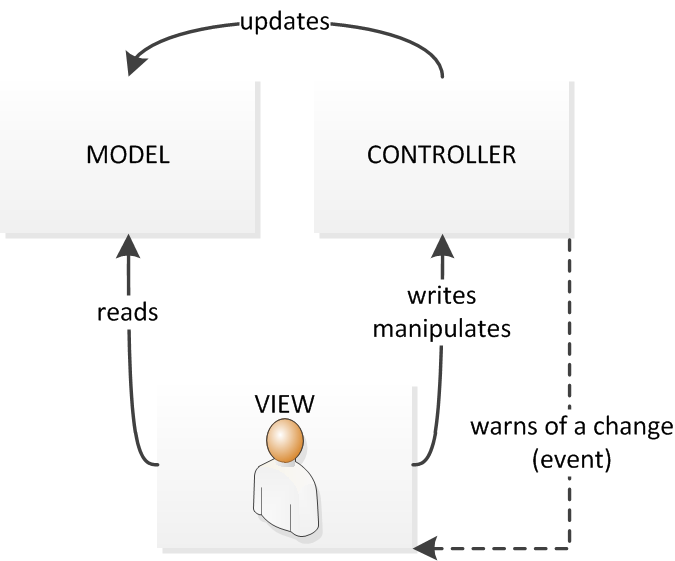
\includegraphics[scale = 0.8, natwidth = 50, natheight = 50]{modele-mvc.png} 
	\end{center}
	\begin{quote}
	Le pattern MVC (Modele - Vue - Controller) est un modèle destiné à répondre aux besoins des applications
	interactives en séparant les problématiques liées aux différents composants au sein de leur architecture respective
	\textit{(Wikipedia)}
	\end{quote}
	
	L'integration de ce pattern au sein du projet est donc approprié.\\
	Lorsque l'utilisateur appuis sur un bouton, le listener (Controller) est appelé puis le model update les données
	pour ensuite notifier la vue des changements graphique à effectuer.

\end{document}
